\documentclass{bhcguides}

\usepackage[legalpaper, portrait, margin=1.2in]{geometry}
\usepackage[utf8]{inputenc}
\usepackage{tabu}
\setlength{\parindent}{0pt}
\setlength{\parskip}{6 pt}

\usepackage{graphicx}
\graphicspath{ {images/} }

\usepackage{url}
\usepackage{hyperref}
\usepackage{cite}

\begin{document}

\title{Volunteer Manual}

\includegraphics[width=1.0\textwidth]{BHCbanner.png}
\date{\today}
\maketitle

\tableofcontents

\section{Overview}

The Building Healthy Communities programme is a partnership that delivers a range of initiatives, activities, interventions and skills classes to improve the well-being of the community as a whole, and also the members of that community. As a volunteer, you contribute in running these initiatives. But if you've come this far, you already know that. What this website got to do with anything and how do I use it? That is where this manual comes in.

The Building Healthy Communities website is a fast, convenient way for you to access details about the initiatives you are either attending or supervising, information about the sessions and ways for you to add new meetings and take attendance. The website also features contact details and a way to request changes to your own details, contact or otherwise. This manual will walk you through the process of logging in, viewing your details and initiatives and doing all the other things listed above. It will also give additional guides on how to contact staff members and the steps needed to be undertaken in the case of loosing your login details.

\pagebreak

\section{System Access and Login}
\label{sec:syslogin}

The website can be accessed through most major web browsers (Chrome, Firefox, Safari, IE8 or higher). Before accessing the site, you should have your email address and password (given to you by an administrator) on hand. Upon entering the website, you will be taken to the login page, as seen in \autoref{fig:initialLogin}.

\begin{figure}[h!]
 \centerline{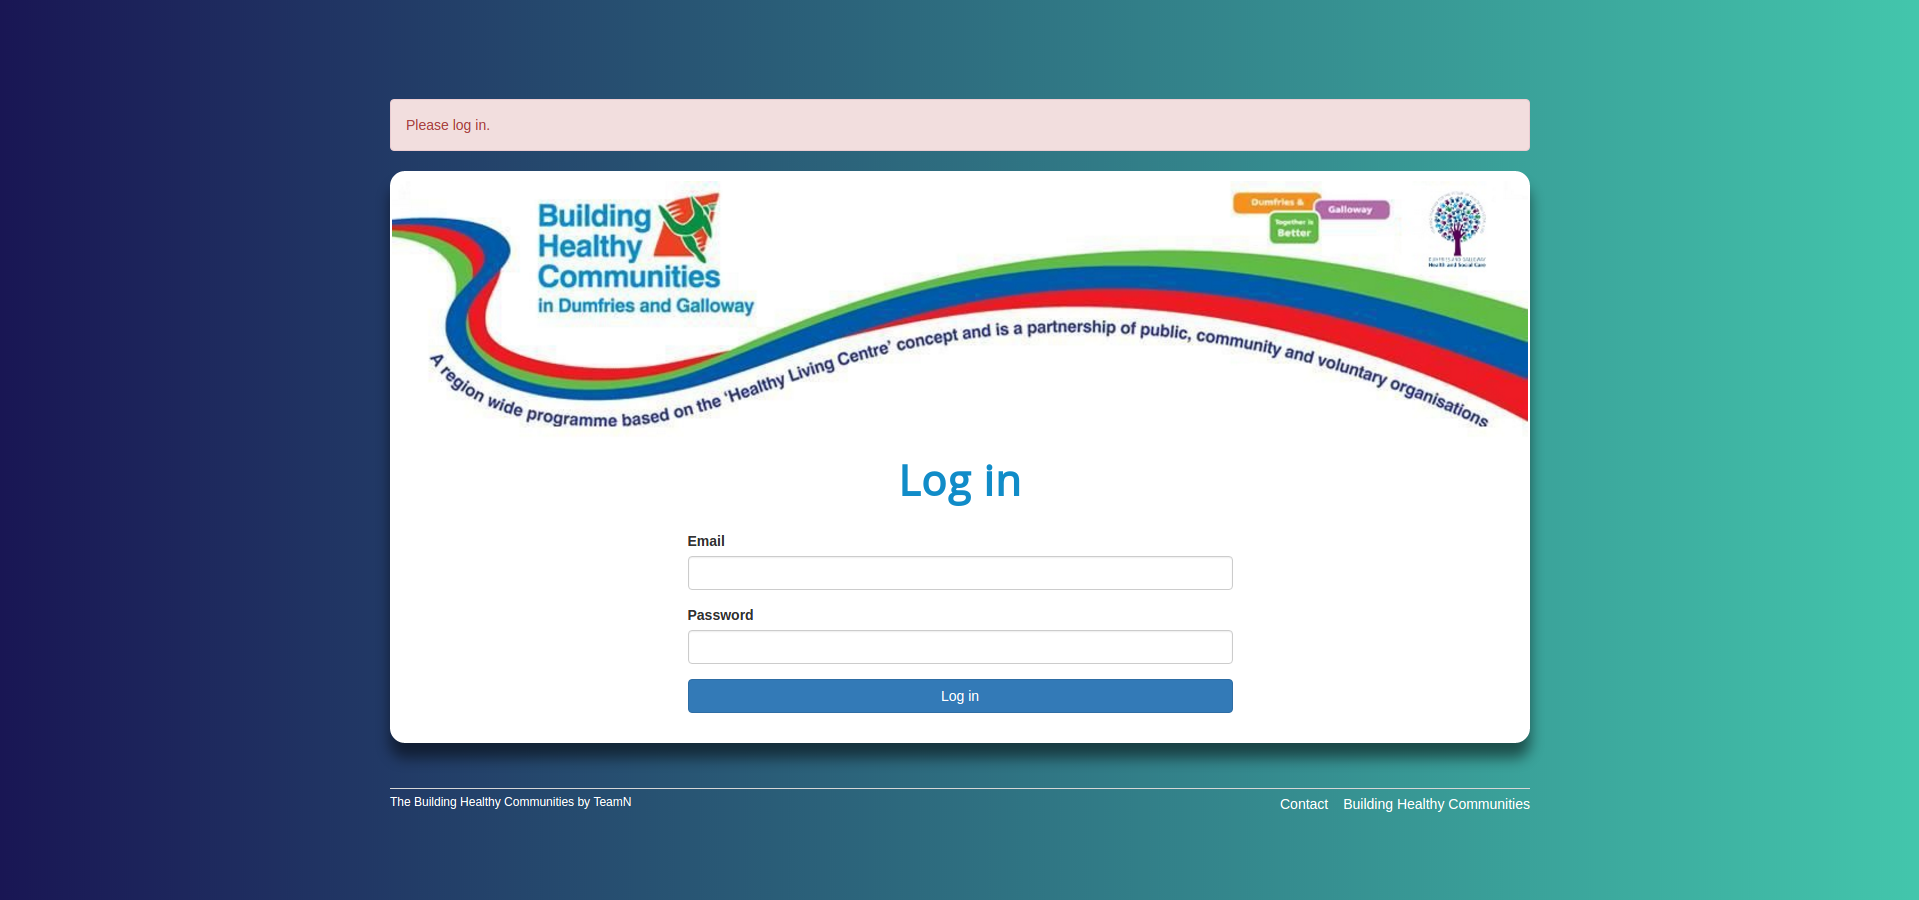
\includegraphics[width=\textwidth, height=\textheight, keepaspectratio]{loginscreen.png}}
 \caption{Login page}
 \label{fig:initialLogin}
\end{figure}

To login to the website, enter your email address and password. Until you do so, there is no way to access the website beyond this page. In the case that you have forgotten your email address and/or password, see \autoref{sec:contacts}: Contacts and Forgotten Passwords.

\pagebreak

\section{Home Page}
\label{sec:homepage}

Once logged in to the system, you will be presented with the home page, as seen in \autoref{fig:homePage}. From here, you can see an overview of all the initiatives you help to run. You can see the information given includes the initiative name, a brief description, and the location.

The initiative name is a link to the page of that initiative, from which you can view various metrics and details, as well as add new meetings, as detailed in \autoref{sec:initiatives}: Initiative Info and \autoref{sec:meetings}: Meetings.

As a volunteer, you should leave feedback every six months. The button to leave feedback is above the list of initiatives. For more detail see \autoref{sec:feedback}: Feedback.

Finally, at the top of the screen is the menu bar, seen in \autoref{fig:menuBar}. From here you can go between the home page and profile page (\autoref{sec:profile}), or log out.

\begin{figure}[h]
 \centerline{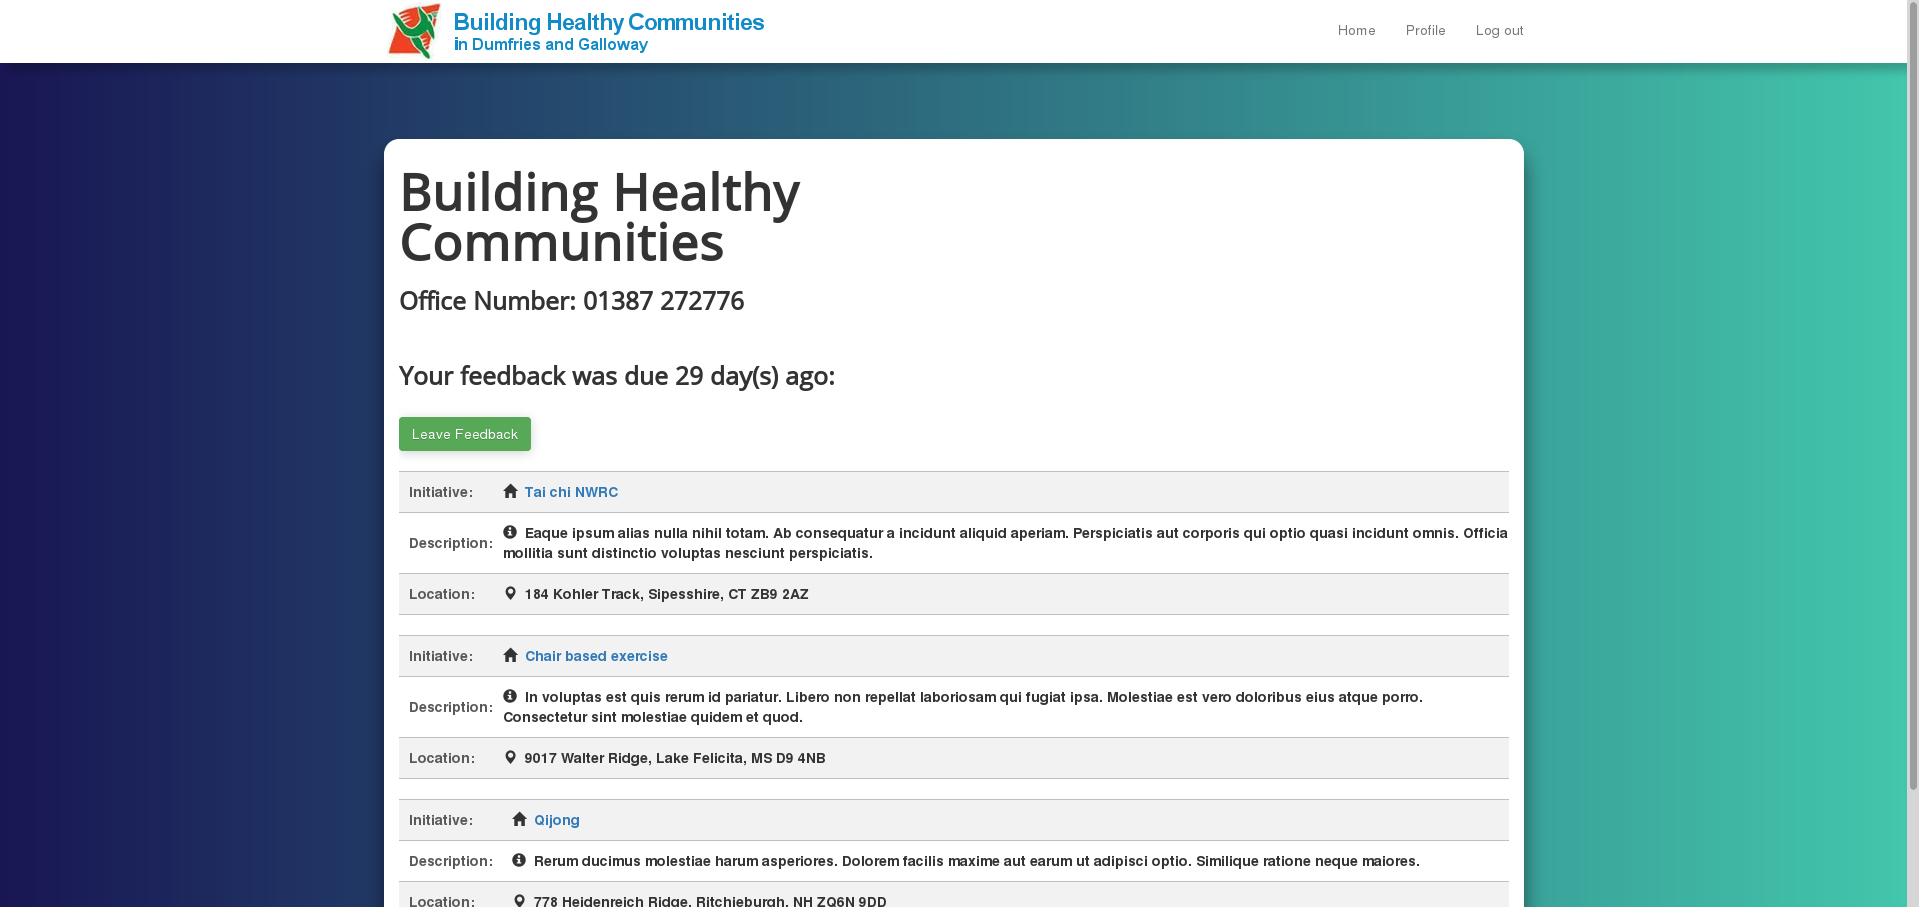
\includegraphics[width=\textwidth, height=\textheight, keepaspectratio]{homepage.png}}
 \caption{Home page}
 \label{fig:homePage}
\end{figure}

\begin{figure}[h]
 \centerline{
\includegraphics[width=\textwidth, height=\textheight, keepaspectratio]{menubar.png}}
 \caption{Menu bar}
 \label{fig:menuBar}
\end{figure}

\pagebreak

\section{Profile Page and Detail Changes}
\label{sec:profile}

The profile page, seen in \autoref{fig:profilePage} contains all the details the Building Healthy Communities system holds on you, from name and date of birth, to emergency contacts or the direct funding you receive. As this data is protected, only you and system administrators can view it. However, you cannot modify this information yourself, though you may send a request for an admin to change it. 

To do this, click the blue 'Change Details' button near the top right of the page. This will take you to a small text box page (\autoref{fig:detailChange}) where you may type in the details that you want to be changed, and what you want them changing to. In case of incorrect details you can always cancel your request. This can by done by visiting your homepage, scroll down to the "Open Service Request" section and delete your desired request. An example can be shown in (\autoref{fig:detailDelete}).

\begin{figure}[h]
 \centerline{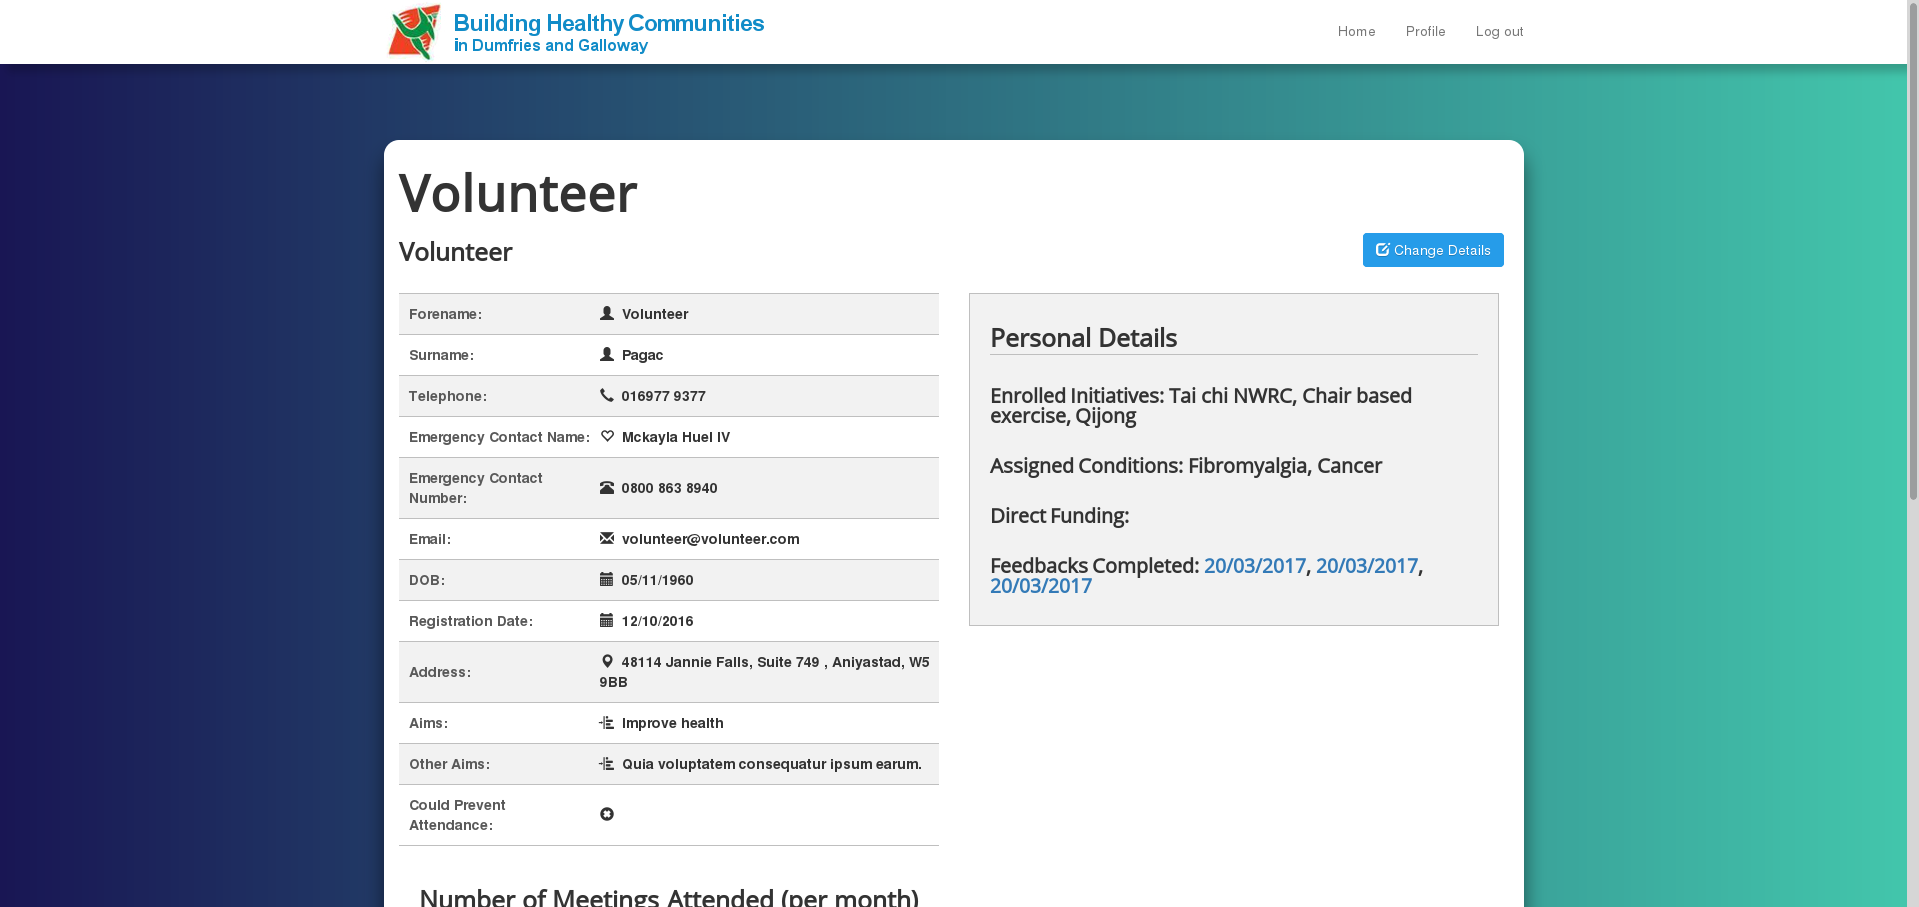
\includegraphics[width=\textwidth, height=\textheight, keepaspectratio]{profilepage.png}}
 \caption{Profile page}
 \label{fig:profilePage}
\end{figure}

\begin{figure}[h]
 \centerline{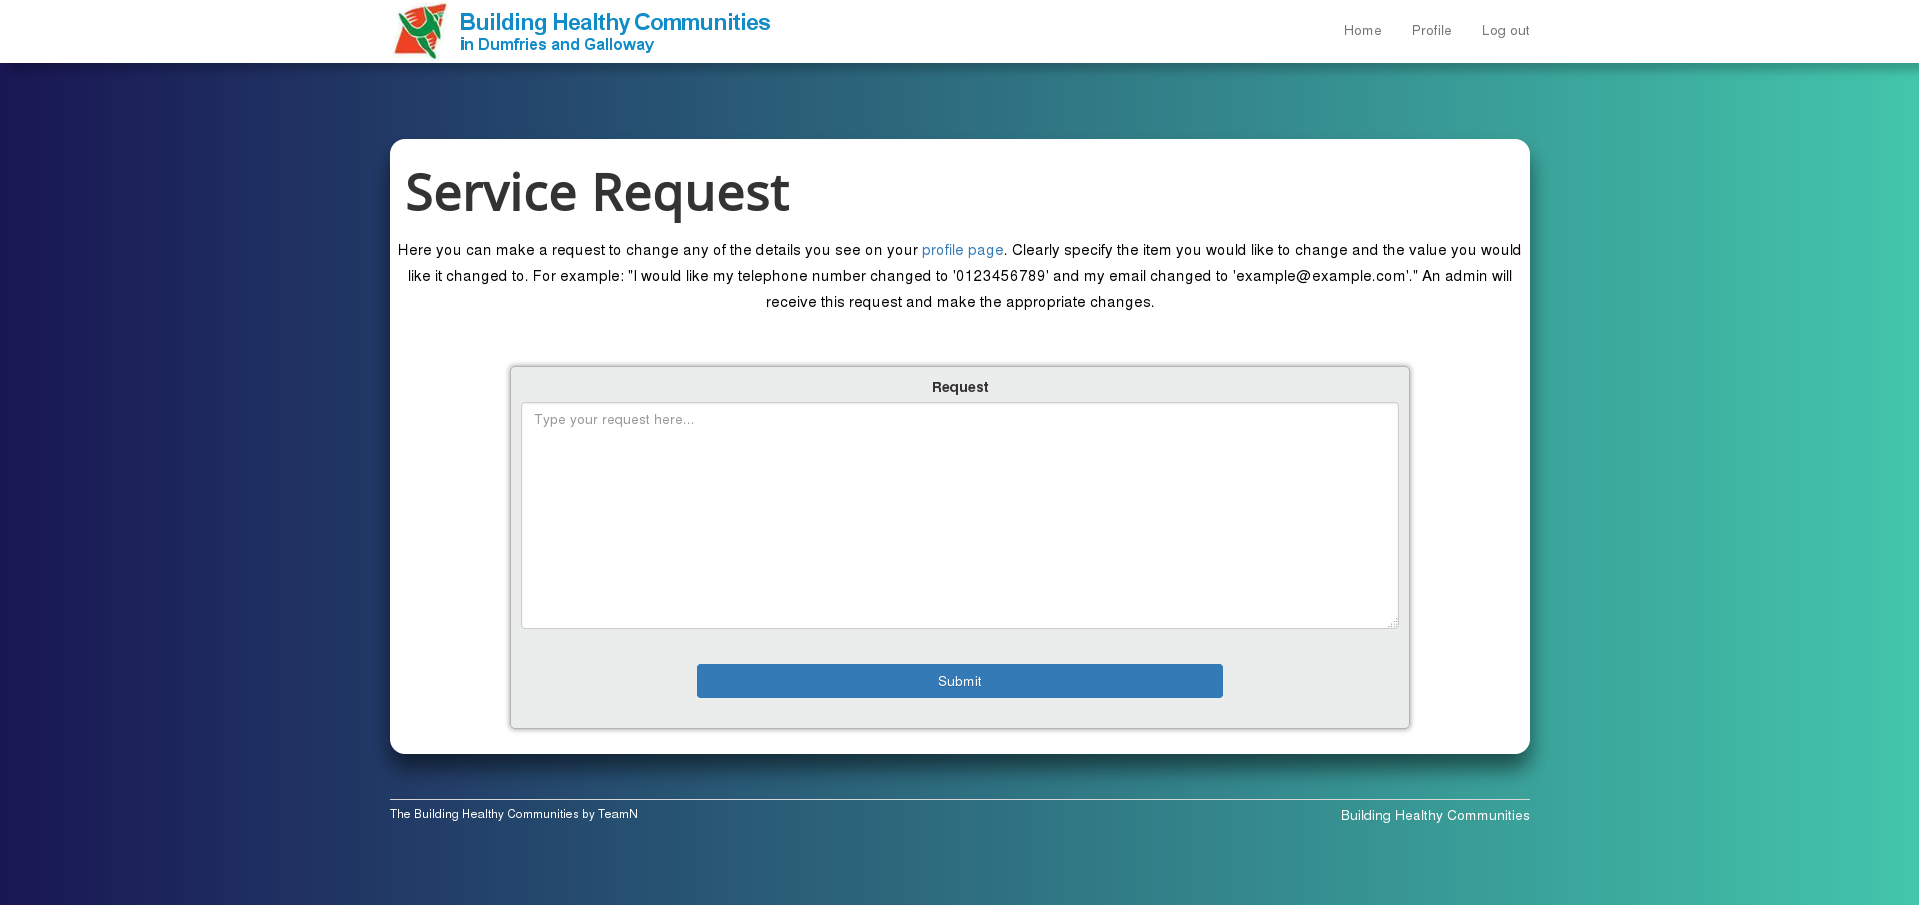
\includegraphics[width=\textwidth, height=\textheight, keepaspectratio]{detailchange.png}}
 \caption{Changing details request}
 \label{fig:detailChange}
\end{figure}

\begin{figure}[h]
 \centerline{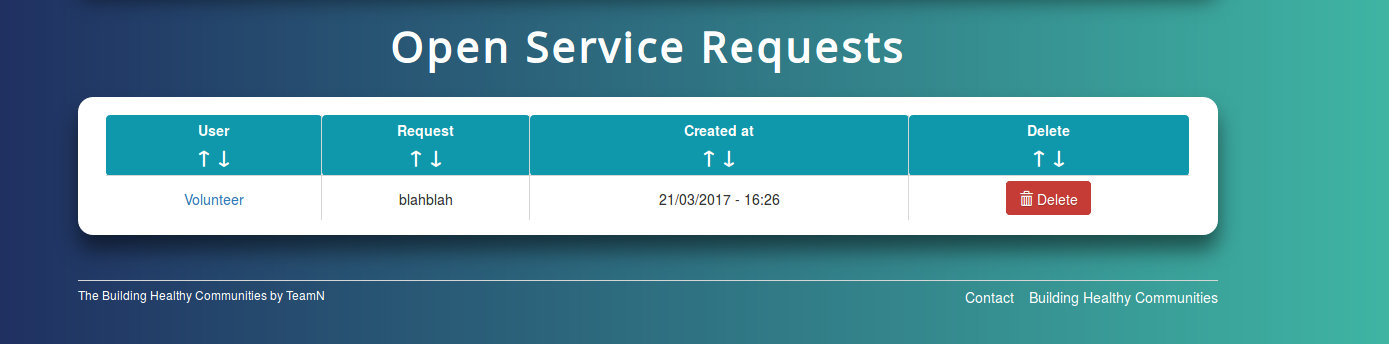
\includegraphics[width=\textwidth, height=\textheight, keepaspectratio]{deleteRequest.png}}
 \caption{Delete details request}
 \label{fig:detailDelete}
\end{figure}

\section{Initiative Information}
\label{sec:initiatives}

The initiatives are the lifeblood of the BHC programme. As a volunteer, it is your job to run these initiatives, and it is from this page, seen in \autoref{fig:initiativePage} that you can view the various details necessary for this upkeep, add new sessions, and take attendance. To access the initiative page for a particular initiative, click its name on your home page.

The details visible from this page include:
\begin{itemize}
	\item Initiative name and area
	\item Initiative location
	\item A brief description
	\item The most recent meeting
	\item Number of enrolled members
	\item Number of funders
	\item Total meetings
	\item Average attendance
	\item Members unenrolled
	\item List of direct funding partners
	\item A graph of average attendance per meeting
\end{itemize}

On the right hand side of the page, you can see a second section, seen in \autoref{fig:fundingInfo}. This lists all the indirect funding that the BHC programme receives related to your attendance. Indirect funding is received from various sources, either to fund a specific initiative (listed on the left), or to go towards initiatives geared towards those with particular conditions in the hope of improving their lives (listed on the right).

\begin{figure}[h]
 \centerline{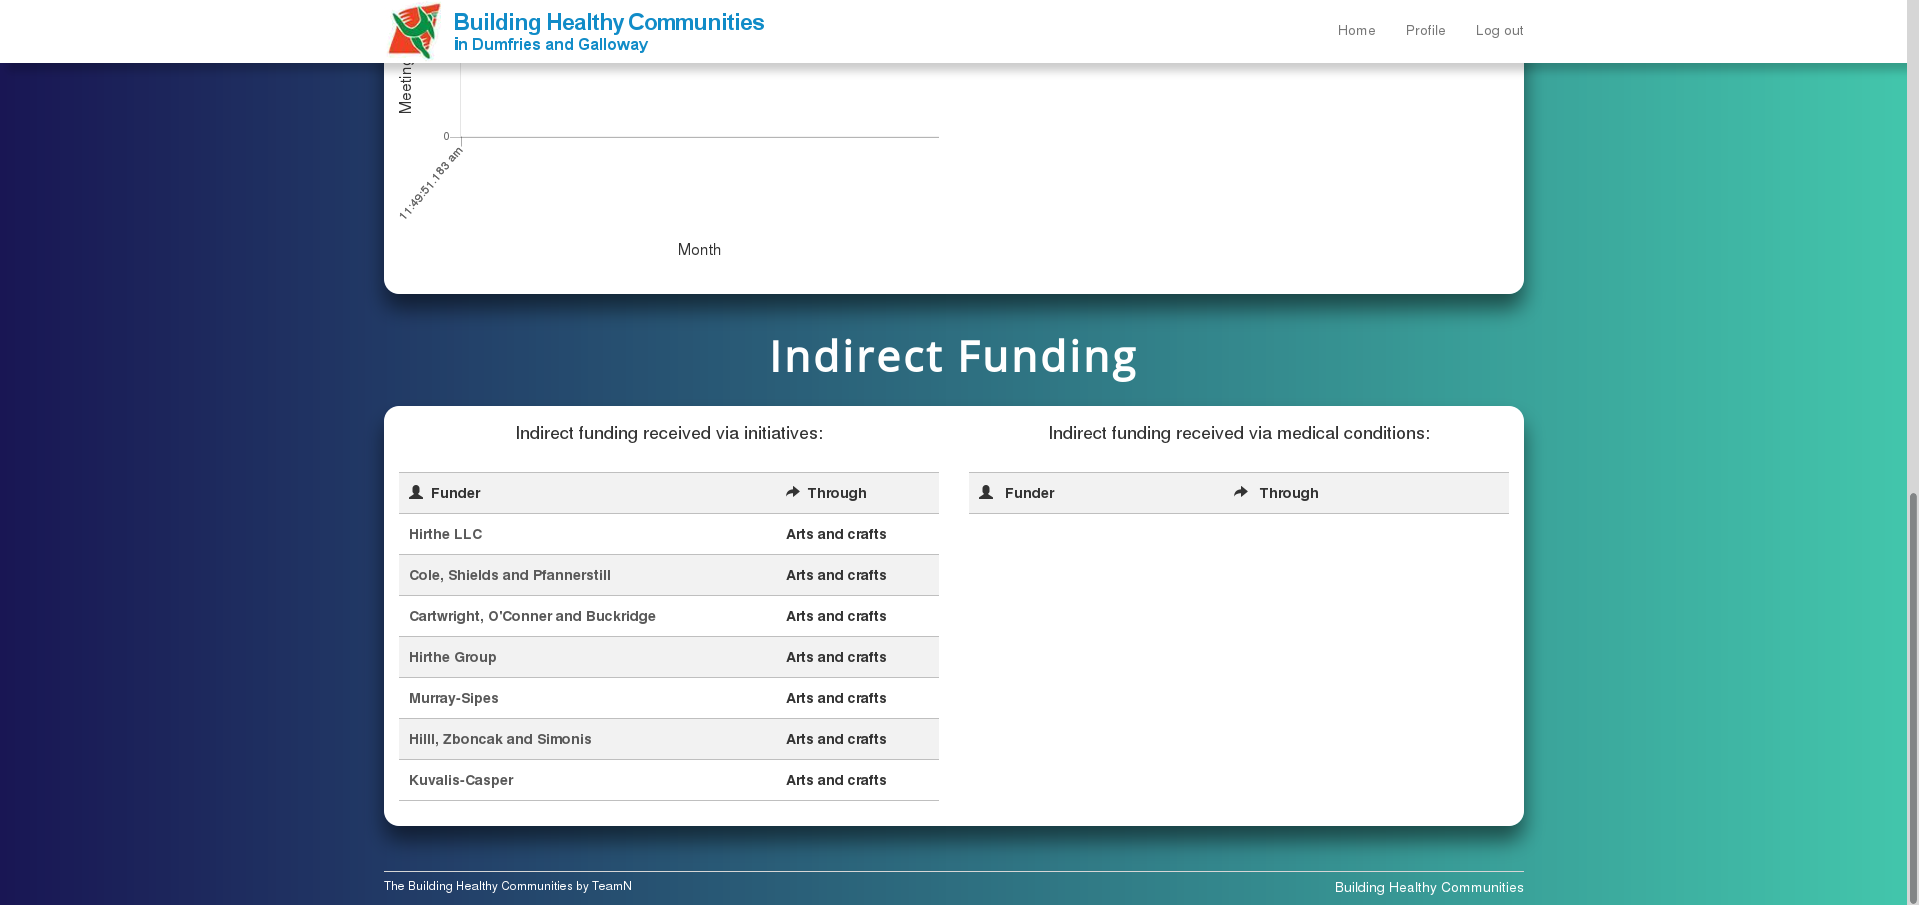
\includegraphics[width=\textwidth, height=\textheight, keepaspectratio]{fundinginfo.png}}
 \caption{Indirect funding info}
 \label{fig:fundingInfo}
\end{figure}

 Further down the page, seen in \autoref{fig:memsandmeets}, a list of attending members along with emergency details can be seen, and further yet (also \autoref{fig:memsandmeets}) a list of all meetings, scheduled and past. Clicking the date of a meeting will take you to the page for that meeting, and clicking the 'New Session' near the top of the page will allow you to create a new session, both of which are described in detail in \autoref{sec:meetings}: Meetings.

\begin{figure}[h]
 \centerline{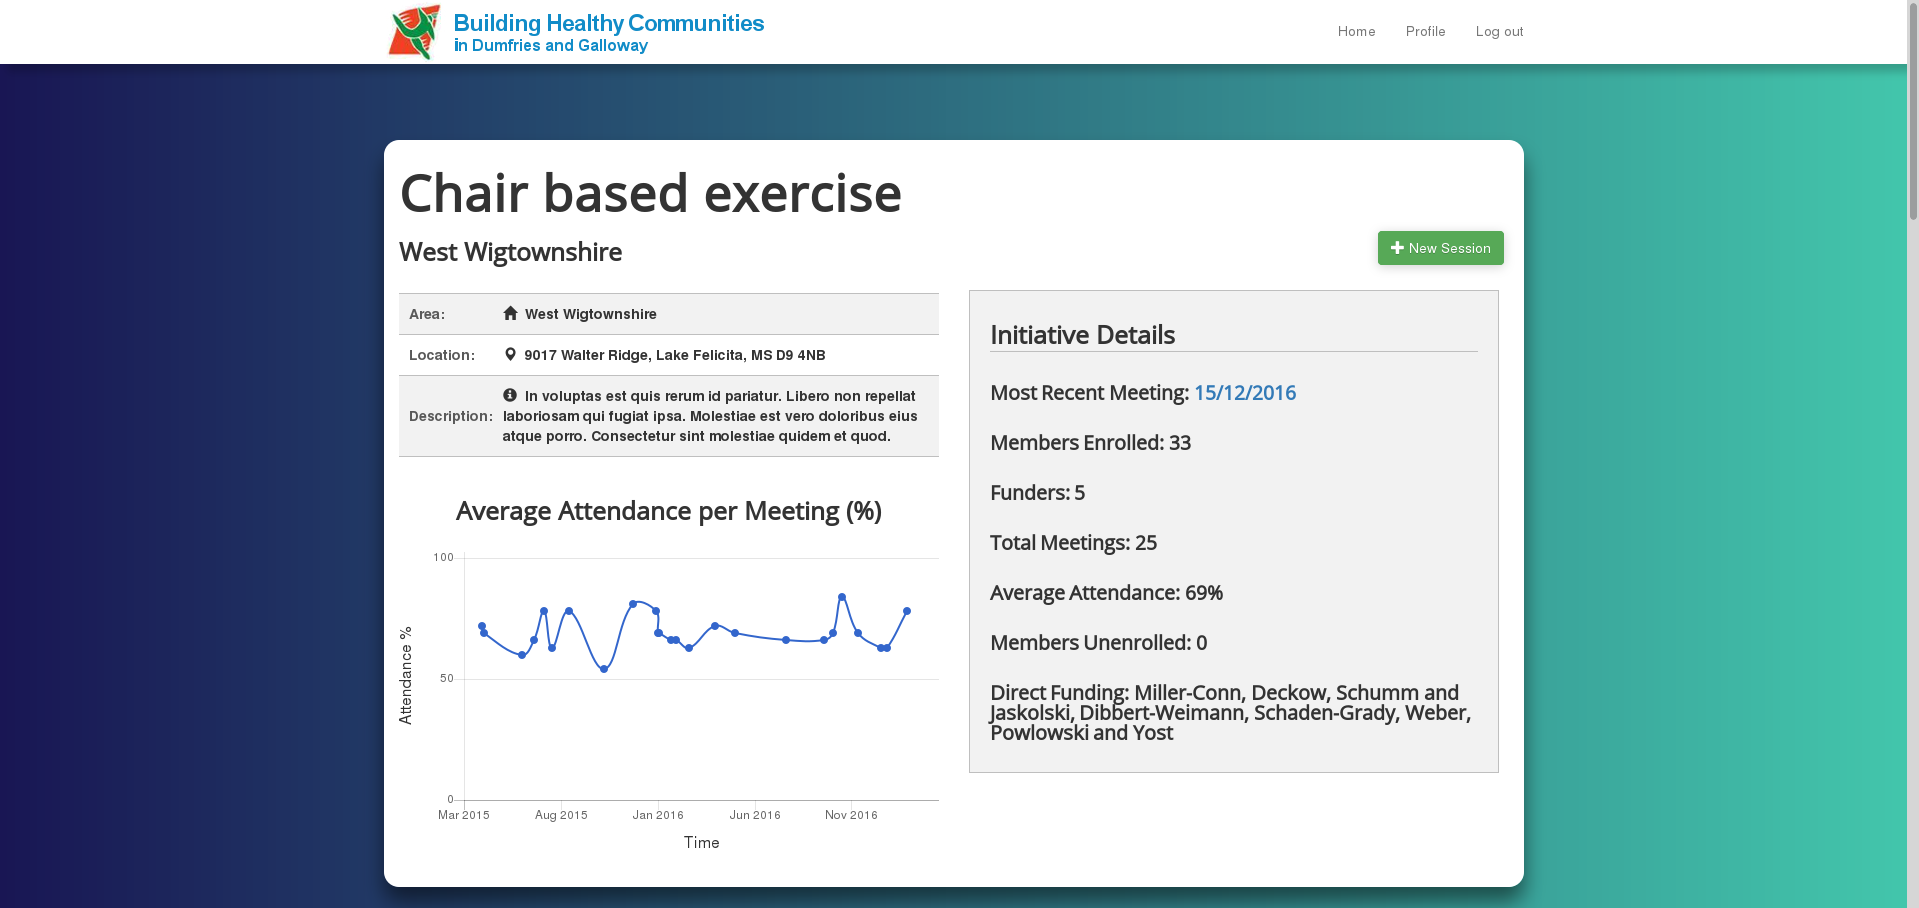
\includegraphics[width=\textwidth, height=\textheight, keepaspectratio]{initiativepage.png}}
 \caption{Initiative page}
 \label{fig:initiativePage}
\end{figure}

\begin{figure}[h]
 \centerline{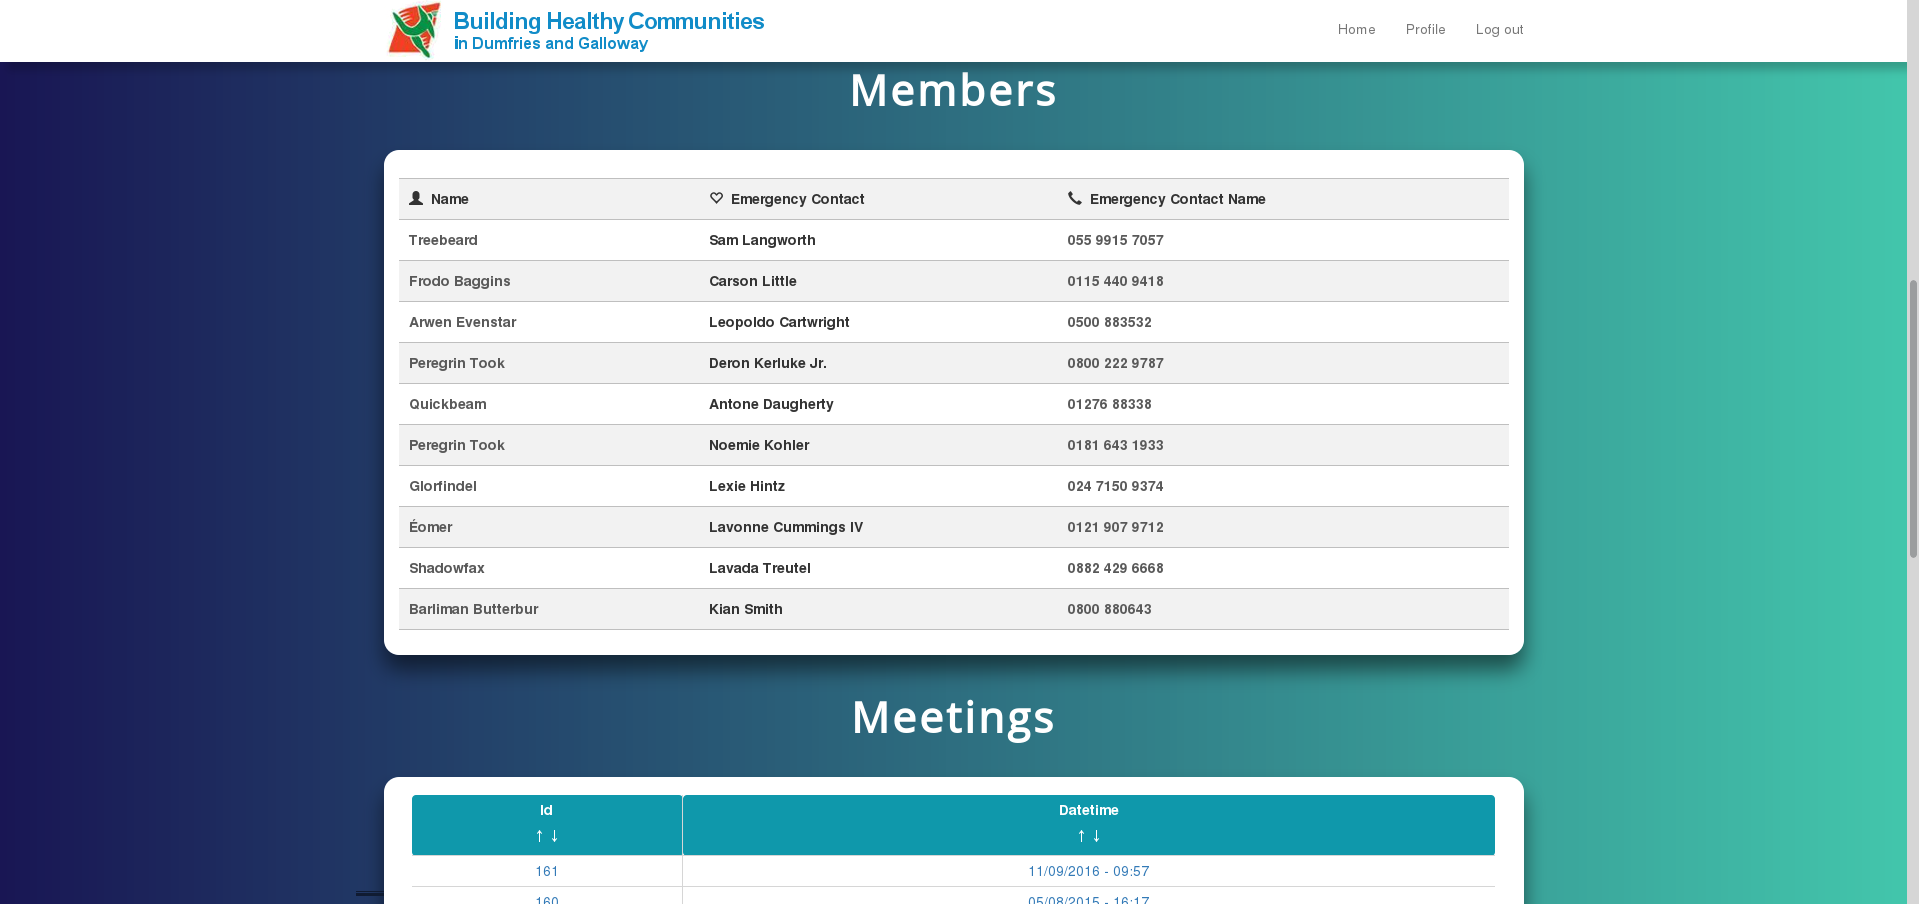
\includegraphics[width=\textwidth, height=\textheight, keepaspectratio]{membersandmeetings.png}}
 \caption{Members and meetings}
 \label{fig:memsandmeets}
\end{figure}

\pagebreak

\section{Meetings}
\label{sec:meetings}

As mentioned above, volunteers such as yourself need to not only view information, but add meetings and take attendance. To add a new session, click the green 'New Session' button near the top right of the page. This will take you to a page titled 'Create a new session', seen in \autoref{fig:newSession}. The drop down menus on this page allow you to create a session. If you click on the new session button, a predefined date scheduled a week after the last scheduled session is already typed for convenience. Although, you can specify any date and time of a session during both the past and future time.

\begin{figure}[h]
 \centerline{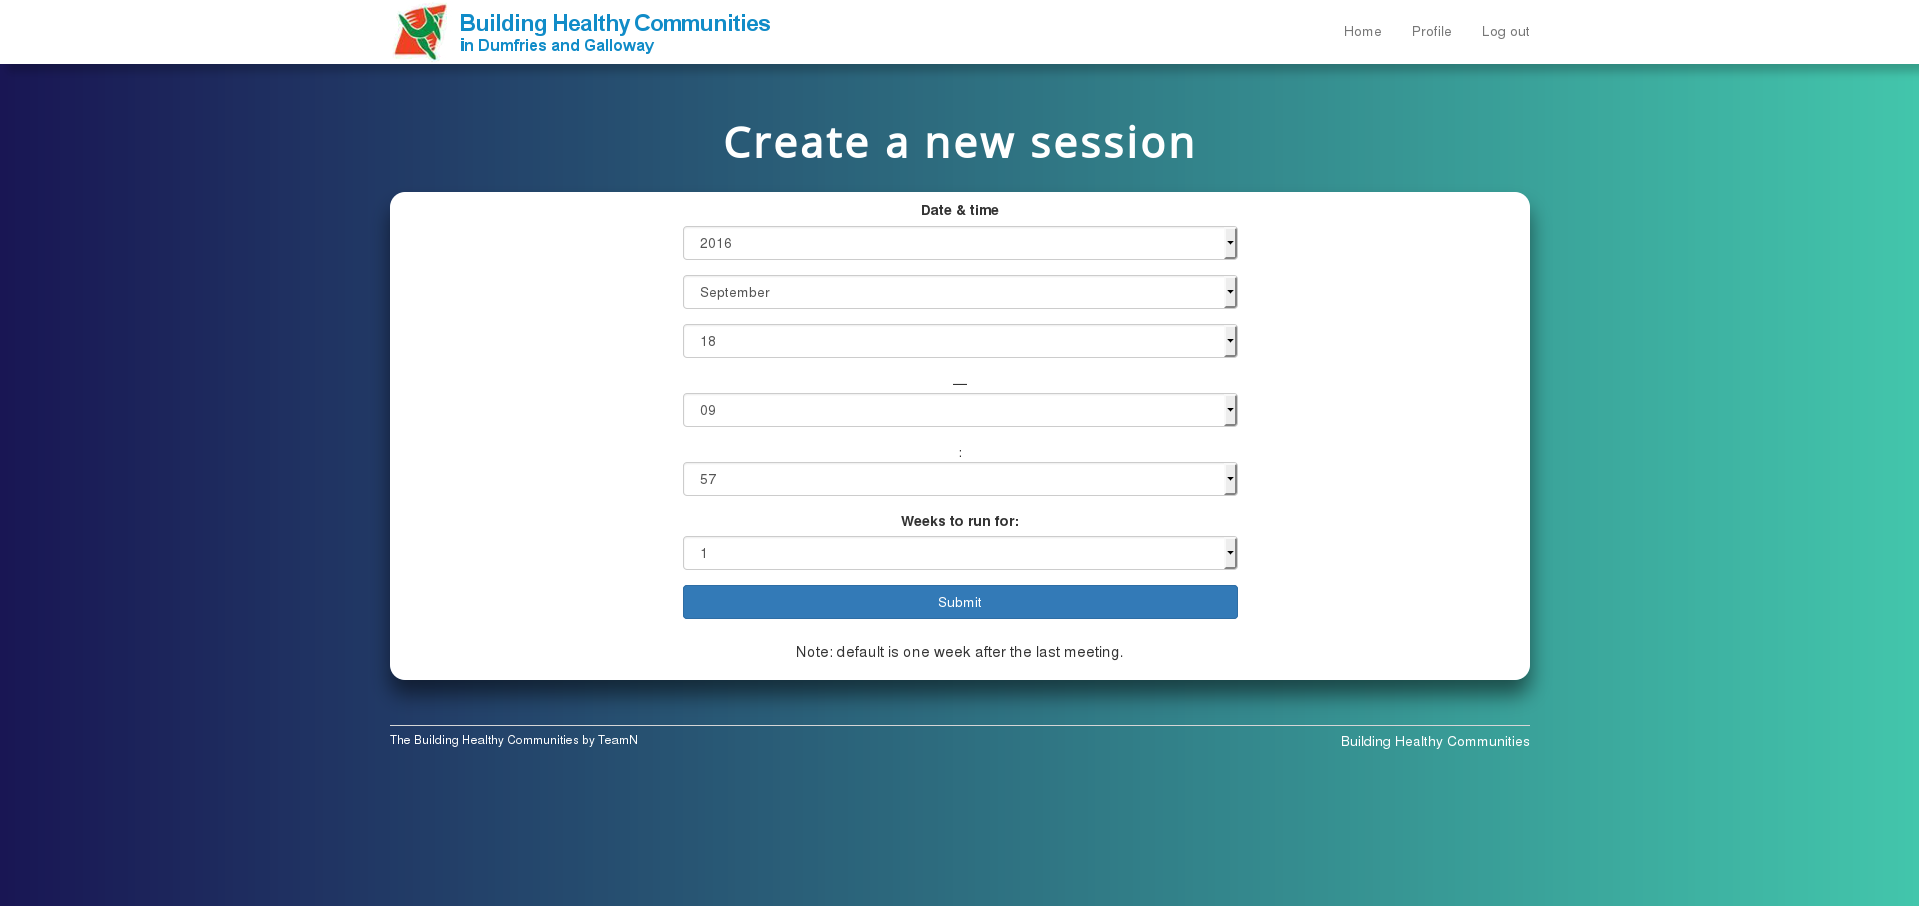
\includegraphics[width=\textwidth, height=\textheight, keepaspectratio]{newsession.png}}
 \caption{Create a new session}
 \label{fig:newSession}
\end{figure}

\pagebreak

The final feature available to you as a volunteer is the ability to view the details of any given meeting for an initiative you help to run and to take attendance for that meeting. To open a meeting page, just click its date or ID anywhere that it appears (in the meetings list, or the most recent meeting). The meeting page shows you a brief overview of the meeting, and a list of all volunteers and service users registered to attend, as seen in \autoref{fig:meetingPage}.

To take attendance, simply tick off the names of those who are in attendance, and click 'Submit' to save the list. This will now load another page (\autoref{fig:meetingAttend}) that displays the percentage of people who attended that session. It is possible to retake attendance, but please note any previous attendance data for the meeting is lost, so be sure you know who is, or was, attending before you select this option!

\begin{figure}[h]
 \centerline{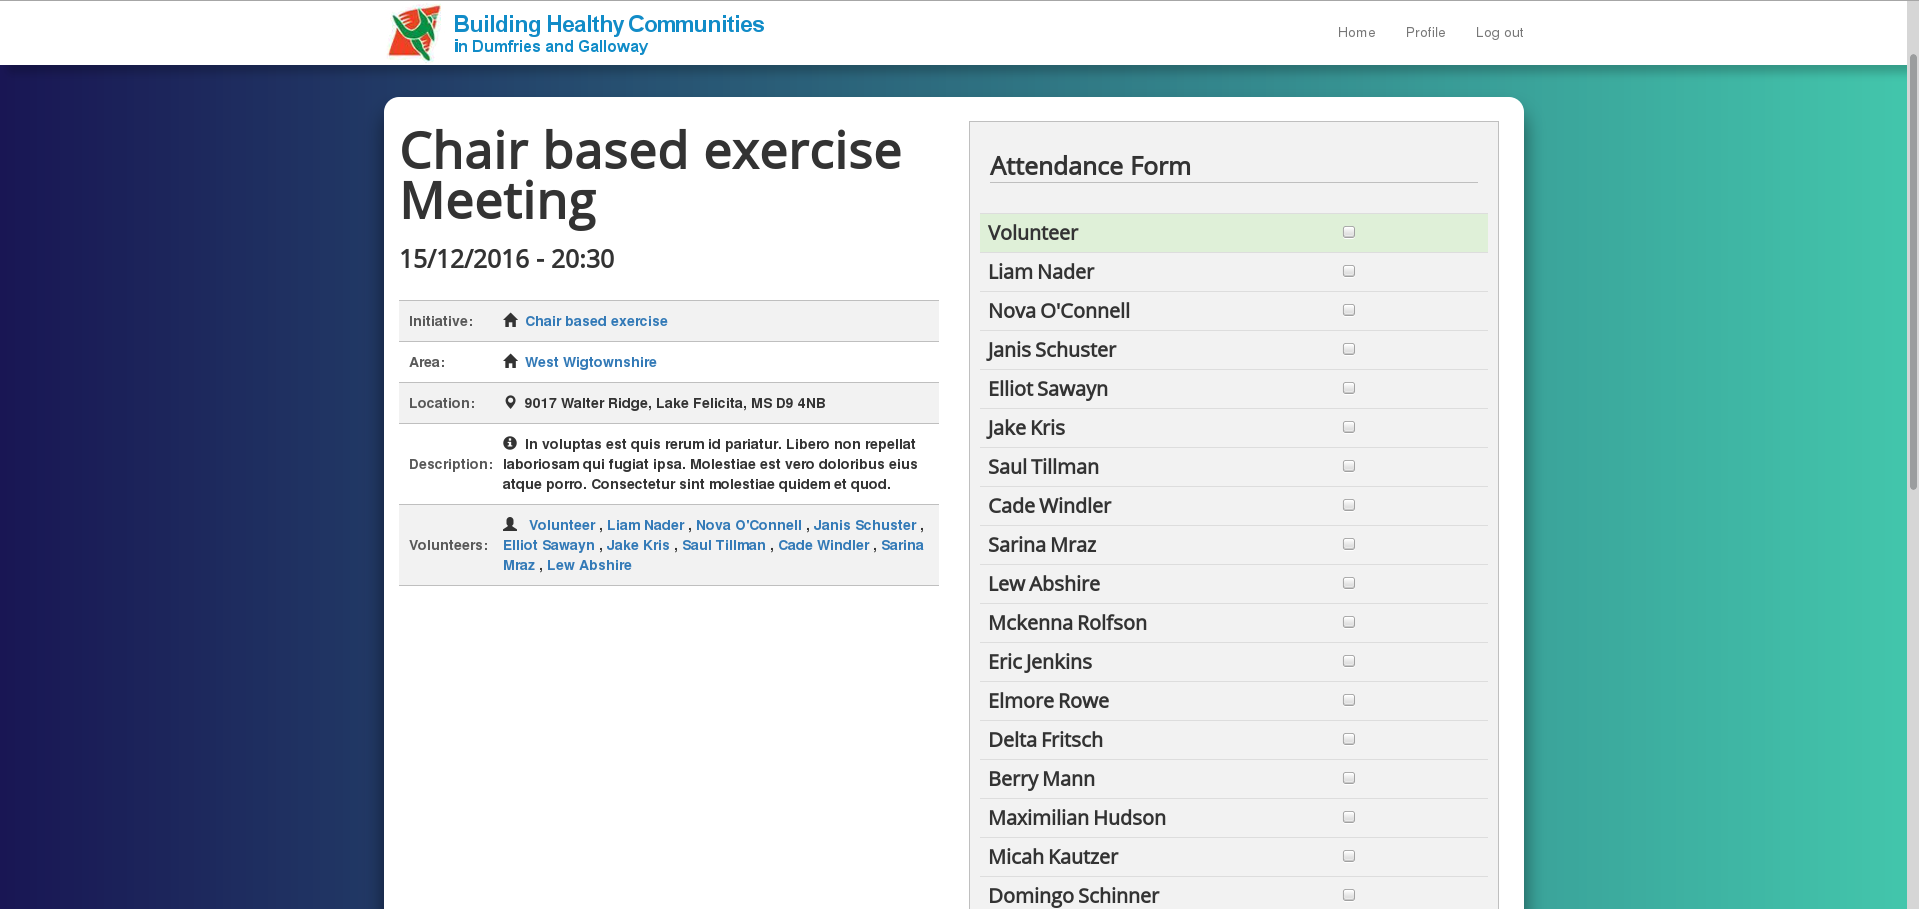
\includegraphics[width=\textwidth, height=\textheight, keepaspectratio]{meetingpage.png}}
 \caption{Meeting page}
 \label{fig:meetingPage}
\end{figure}

\begin{figure}[h]
 \centerline{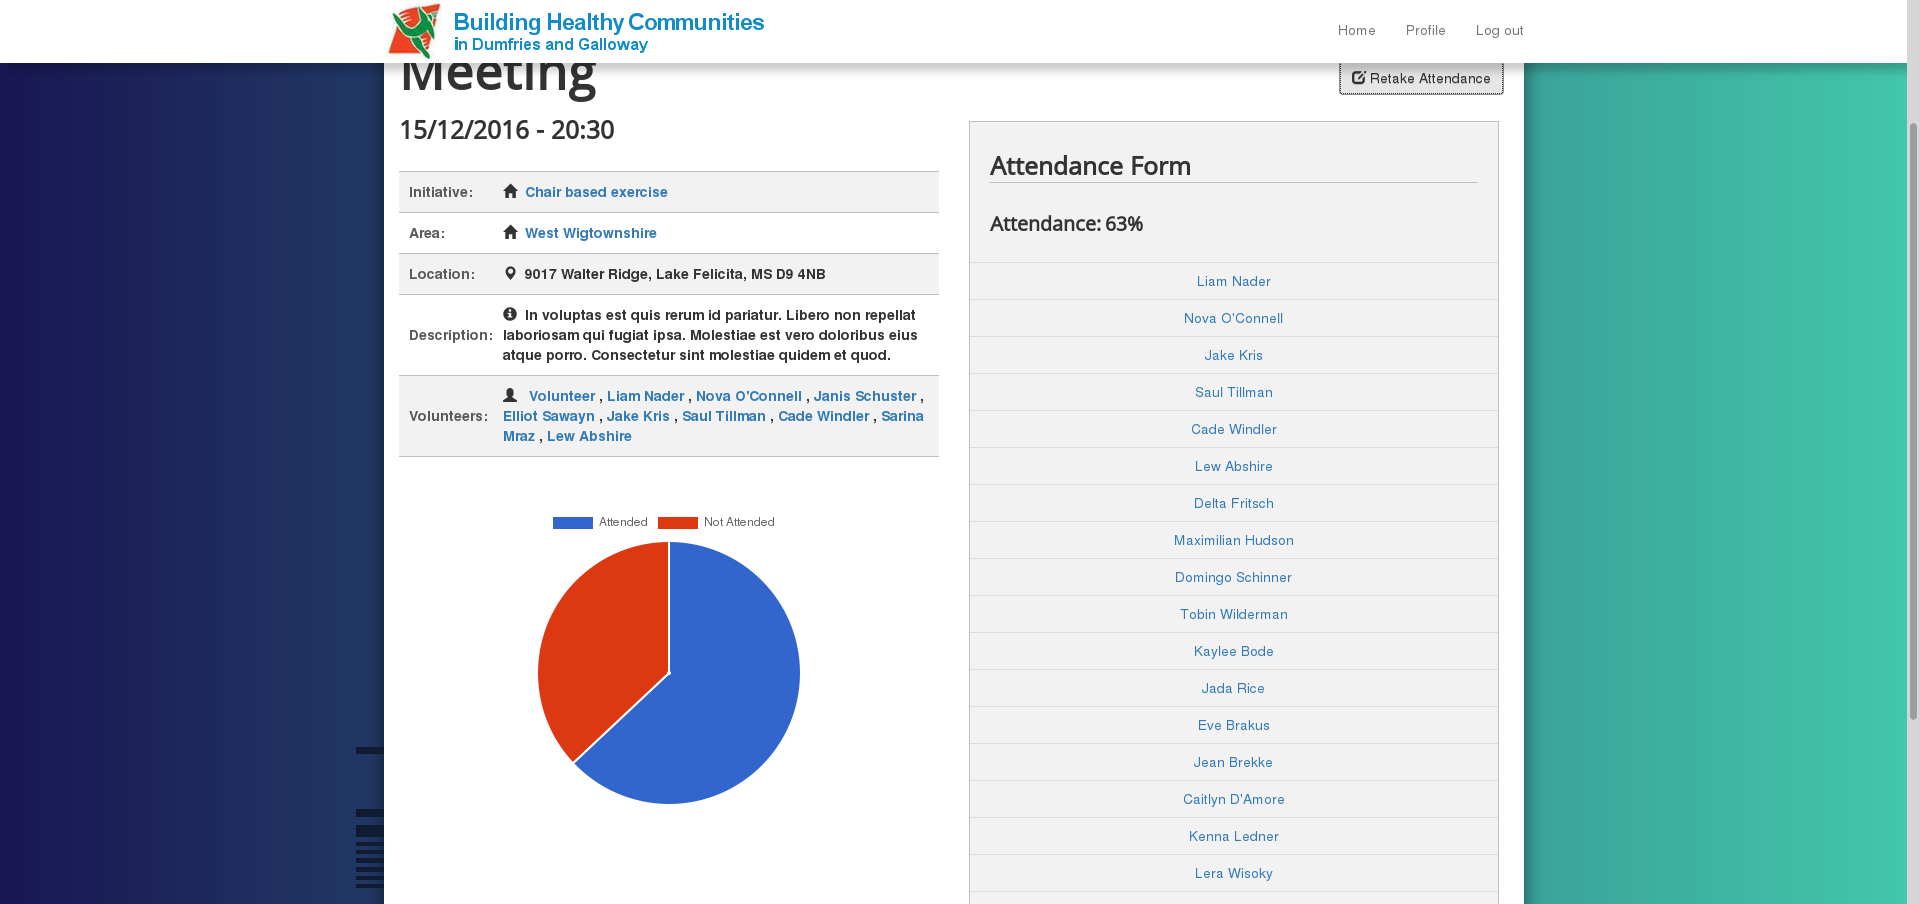
\includegraphics[width=\textwidth, height=\textheight, keepaspectratio]{meetingattendance.png}}
 \caption{Attendance completed}
 \label{fig:meetingAttend}
\end{figure}

\pagebreak

\section{Feedback}
\label{sec:feedback}

Leaving feedback is an important part of the BHC programme. It allows those running the programme to see the progress of everyone involved in the various initiatives, including you as a volunteer. It is advised to submit a feedback at least once every six months, although you may leave feedback at any time. To leave feedback, click the green 'Leave Feedback' button on the home page, and you will be taken to the feedback page, seen in \autoref{fig:feedbackPage}.

The feedback form asks you a standard set of questions about how you have been feeling, and how connected you feel to your community and local area. You can review your feedback anytime you wish which is displayed in the "Feedbacks completed" section at your profile page. The feedback is mainly used for the administrators in an effort to gauge how much the initiatives have affected you, either in a positive or negative way. You should answer the questions honestly, so that the administrators can track your process and help you with any issues raised. The initiatives are there to help, and if they're doing something wrong, or there's something they can do, the BHC programme administrators need to know!

\begin{figure}[h]
 \centerline{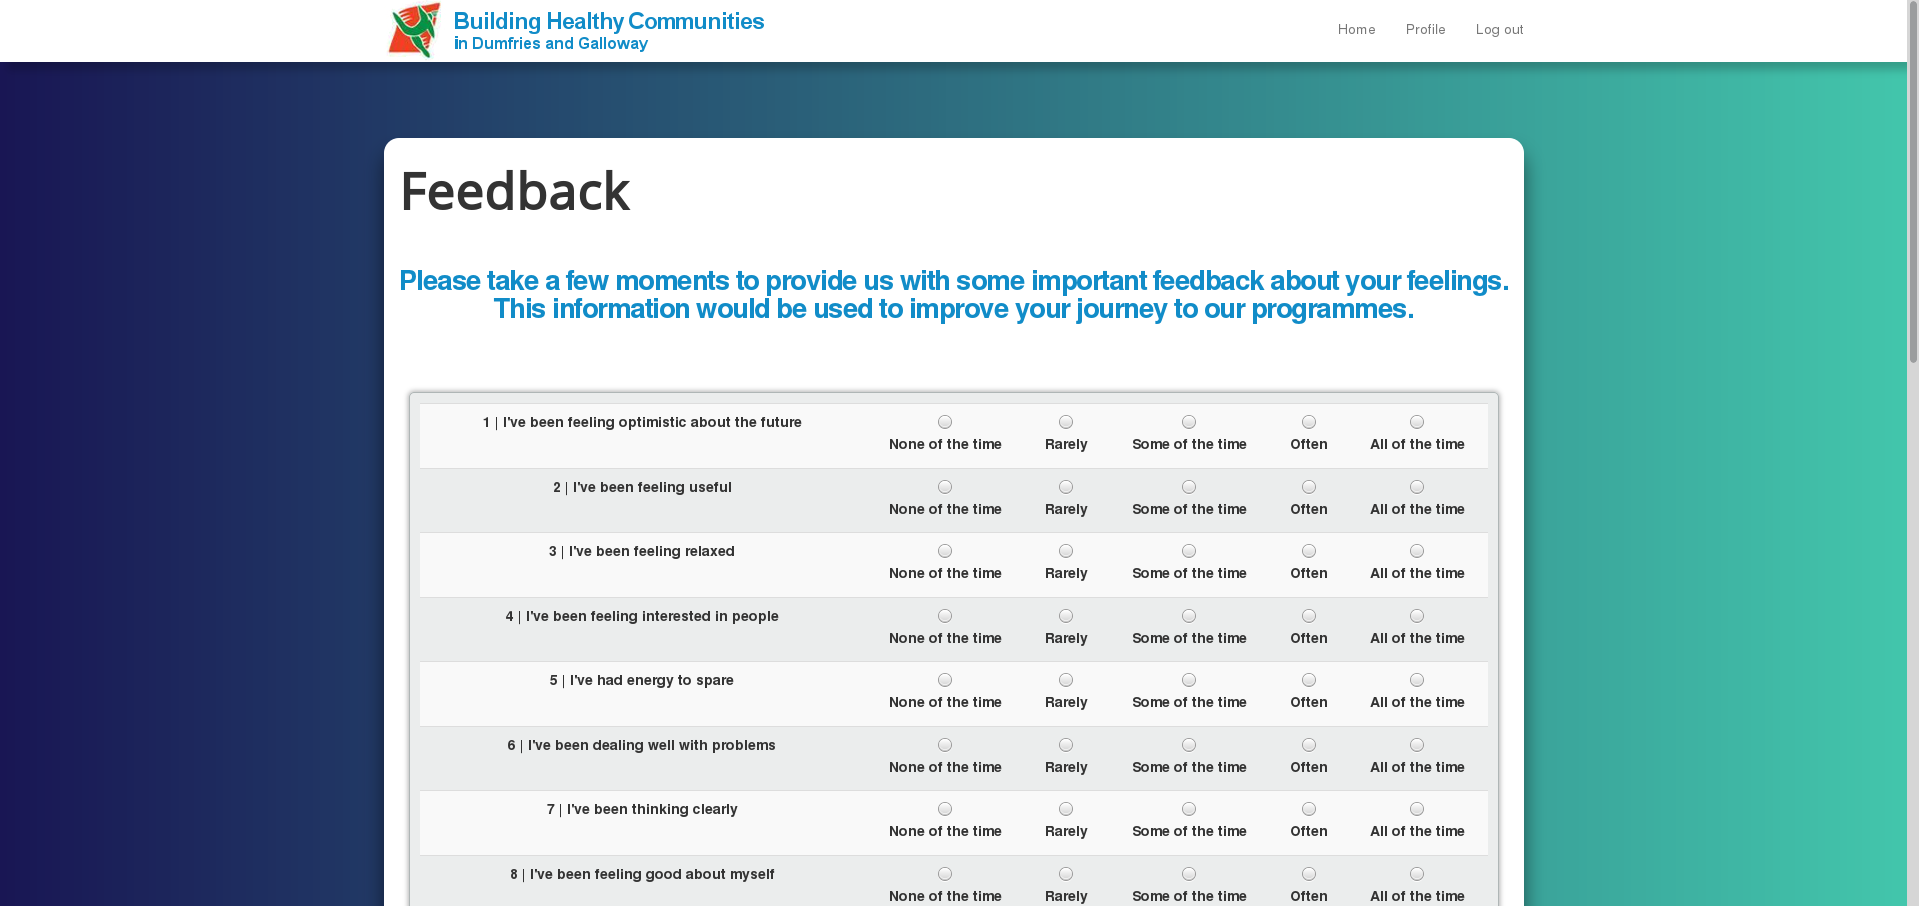
\includegraphics[width=\textwidth, height=\textheight, keepaspectratio]{feedbackpage.png}}
 \caption{Feedback page}
 \label{fig:feedbackPage}
\end{figure}

\section{Contacts and Forgotten Passwords}
\label{sec:contacts}

If you want to find contact details for a given area, there is an easy way to do so. On the bottom right is the word 'Contact'. Clicking on this will bring up the contacts page, from which the addresses of the various area partnerships can be found, as seen in \autoref{fig:contactPage}. This page also includes the names and roles of people working there, and a telephone number. If you have forgotten your email address and/or password, you can call the number for your area and the team will try to help, asking you a few security questions for authentication, before resetting your login details.

\begin{figure}[h]
 \centerline{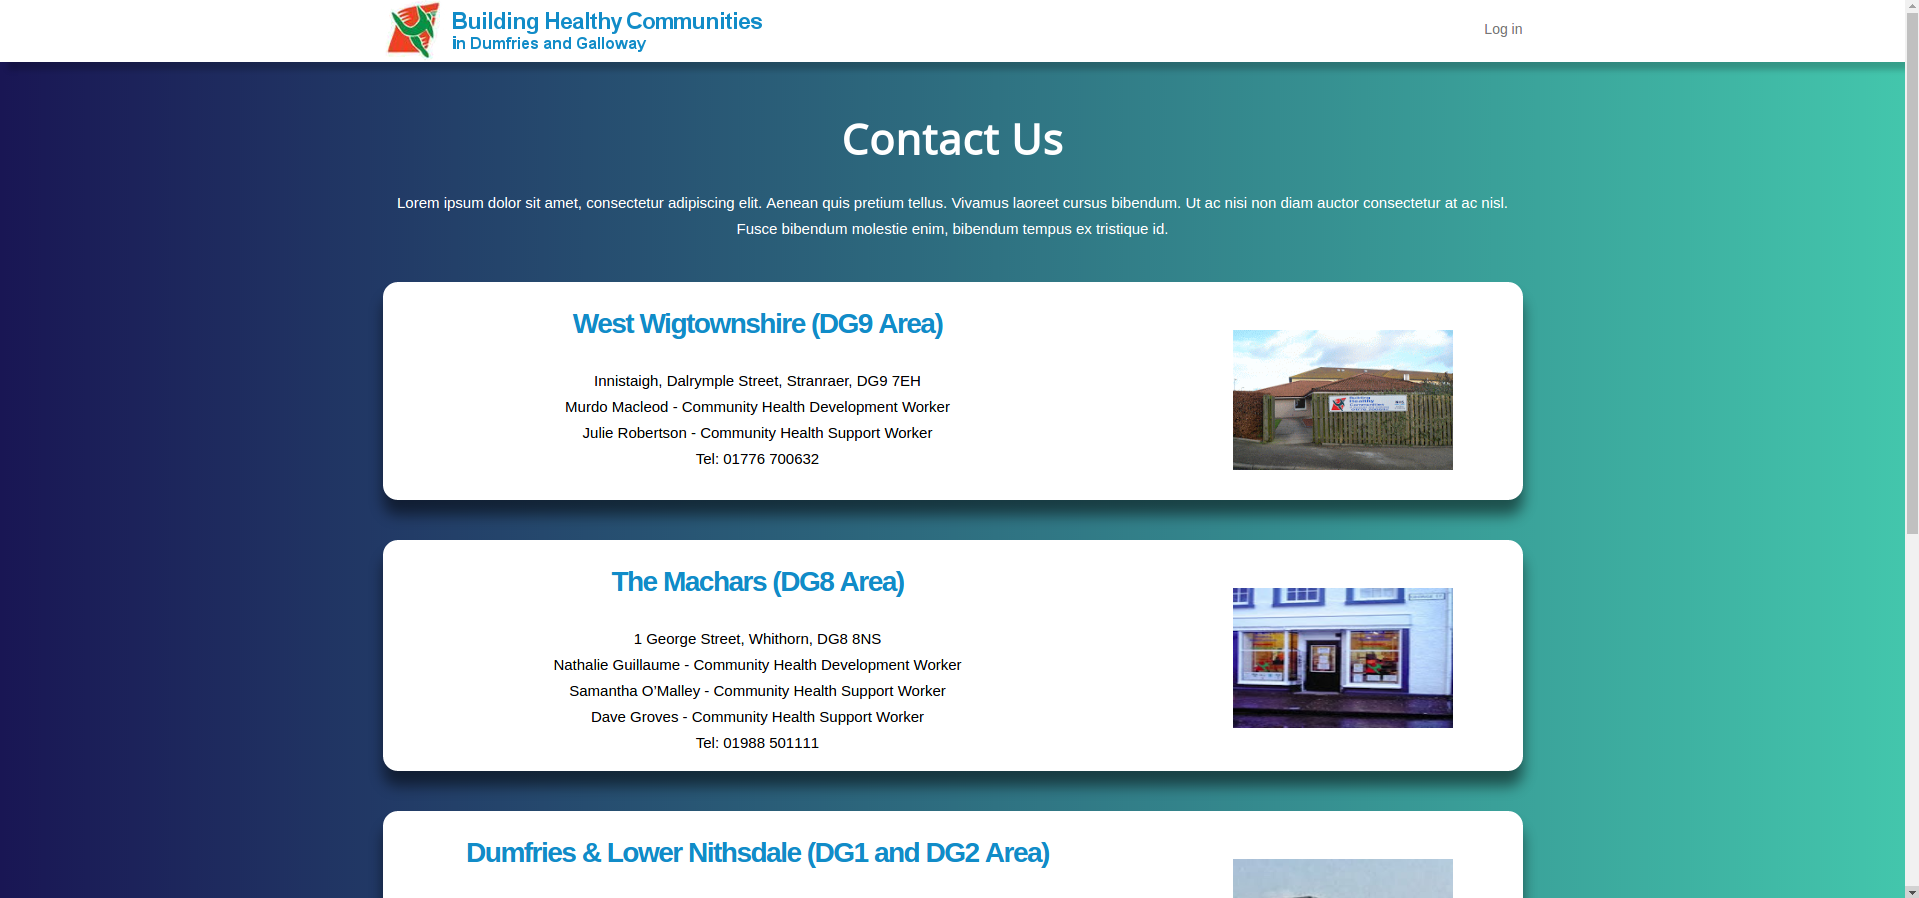
\includegraphics[width=\textwidth, height=\textheight, keepaspectratio]{contactpage.png}}
 \caption{Contact page}
 \label{fig:contactPage}
\end{figure}

\end{document}
